\subsection{Price的计算}
图\ref{fig:sys.param}给出了息票在市场上的价格P和市场上同类息票/债券的年化收益率y之间的定性关系。

\begin{figure}[htbp]
\begin{center}
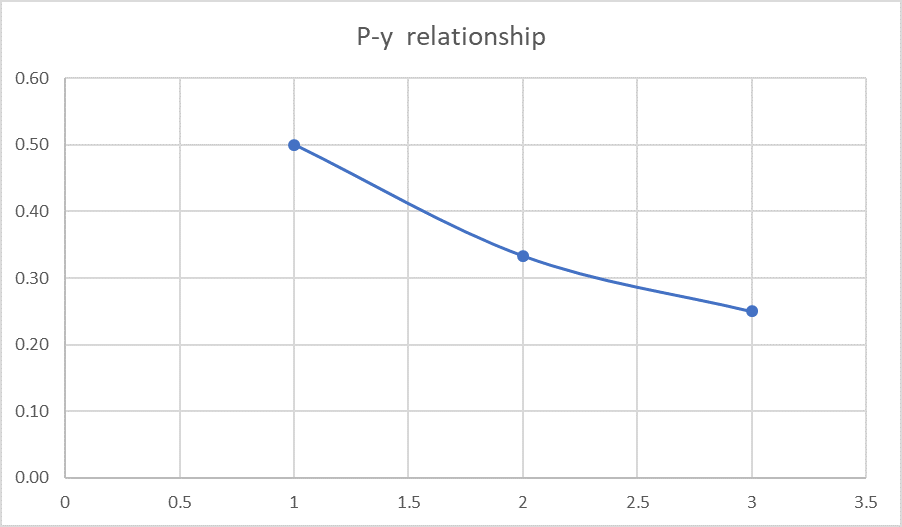
\includegraphics[width=16cm]{img//P_y_Relation.PNG}
\caption{P-y关系图}
\label{fig:sys.param}
\end{center}
\end{figure}

根据泰勒展开式

$P_1 \approx P_0-P_0 \cdot {Duration_D} \cdot (y_1-y_0 )+1/2 \cdot {P_0}\cdot {Convexity_D} \cdot (y_1-y_0 )$

这里的$Duration_D$和$Convexity_D$分别指的是一阶导数和二阶导数,没有除以Price。通过上式,我们可以通过当前息票价格求得未来某时刻息票价格。

\subsection{分期支付利息的计算}
对于一个3年期的息票来说,发行者每年付一次利息,而非到期一次性结清利息。

图\ref{fig:sys.param}给出了一个例子。
\begin{figure}[htbp]
\begin{center}
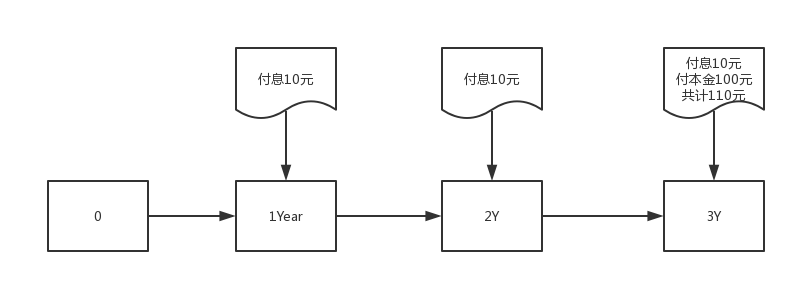
\includegraphics[width=16cm]{img//Interest_Calc.PNG}
\caption{付息日的利息计算}
\label{fig:sys.param}
\end{center}
\end{figure}

假设本金100元,年利率为$10\%$。

$PV=(v*10\%)/{(1+10\%)^1} +{(v*10\%)/(1+10\%)}^2 +{(v*(10\%+1))/(1+10\%)}^3 $

其中,第一项表示第一年付息的现值,第二项表示第二年付息的现值,第三项表示第三年付息和本金的现值。

进一步地,

$PV=(c*v)/f*∑_1^j{1/{(1+y_i/f)}^i +v/{(1+y_n/f)}^n} $

这里,我们把未来的每个现金流折现到今天。

图\ref{fig:sys.param}给出了更进一步的例子。
\begin{figure}[htbp]
\begin{center}
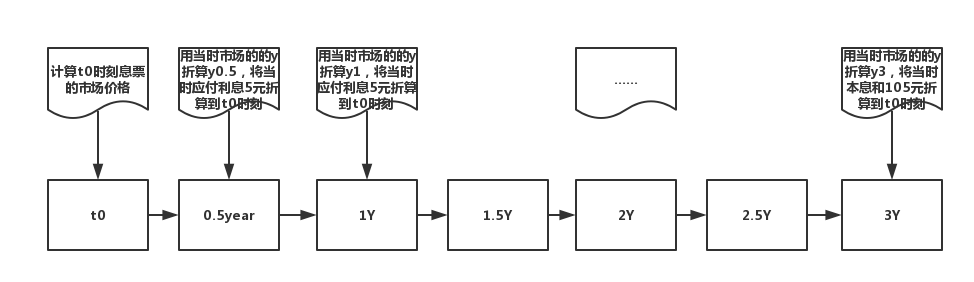
\includegraphics[width=16cm]{img//Interest_Calc_Senior.PNG}
\caption{非付息日的利息计算}
\label{fig:sys.param}
\end{center}
\end{figure}

我们将未来的现金流折现到$t_0$时刻,求得息票在$t_0$时刻的现值后,我们就可以知道应当以多少钱在市场上购入/卖出该息票。这里的$y_0.5, y_1, \cdots y_3$,指的是yield to maturity(到期收益率)。

\subsection{Dirty Price的计算}
图\ref{fig:sys.param}给出了Dirty Price与时间t的关系。
\begin{figure}[htbp]
\begin{center}
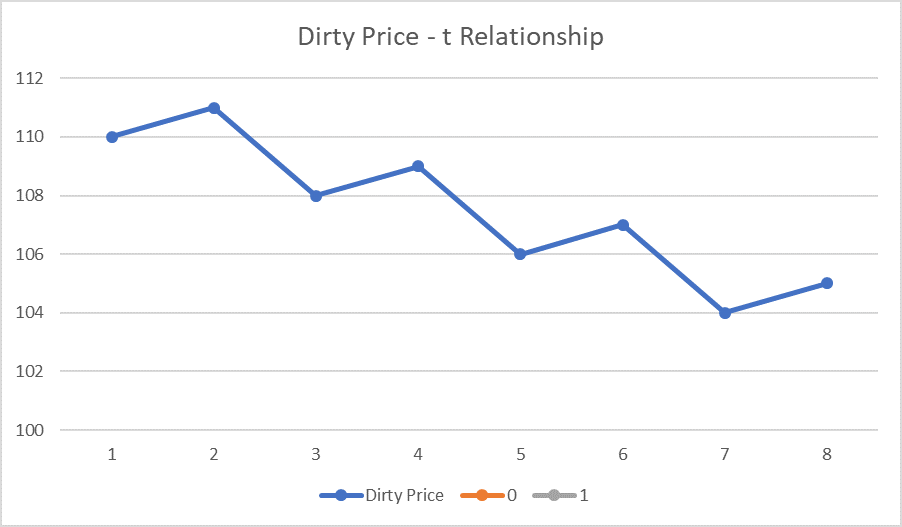
\includegraphics[width=16cm]{img//DirPri_t_Relation.PNG}
\caption{Dirty Price与时间t的关系}
\label{fig:sys.param}
\end{center}
\end{figure}

Dirty price指的是clean price和accrued interest(已经发放的利息)的和。
Clean price指的是还未领取的息票本金折现到当前时刻是多少钱。

其中t坐标轴的偶数(2,4,6,8,……)指的是股息发放日。每次发放股息后,coupon的dirty price等于clean price。随着利息的积累,dirty price逐渐高于clean price,直到下次股息发放日股息再次方法,dirty price再次等于clean price。
市场上的报价通常是clean price,所以交易双方需要根据自己的交易模型计算出accrued interest,在交易时把积累的利息加上去。

对于Duration和convexity,我们有以下结论:
1.Duration的加权平均就是该coupon bond的加权平均
2.Convexity 的加权平均就是该coupon bond的加权平均

规范化表示:
$Duration_avg=(P*V_1*D_1+P*V_2*D_2+ \cdots)/(P*V_1+P*V_2+\cdots)$
$Convexity_avg=(P*V_1*C_1+P*V_2*C_2+\cdots)/(P*V_1+P*V_2+\cdots)$



\subsection{利用牛顿迭代法计算年化收益率}
图\ref{fig:sys.param}表示利用牛顿迭代法计算年化收益率y。
\begin{figure}[htbp]
\begin{center}
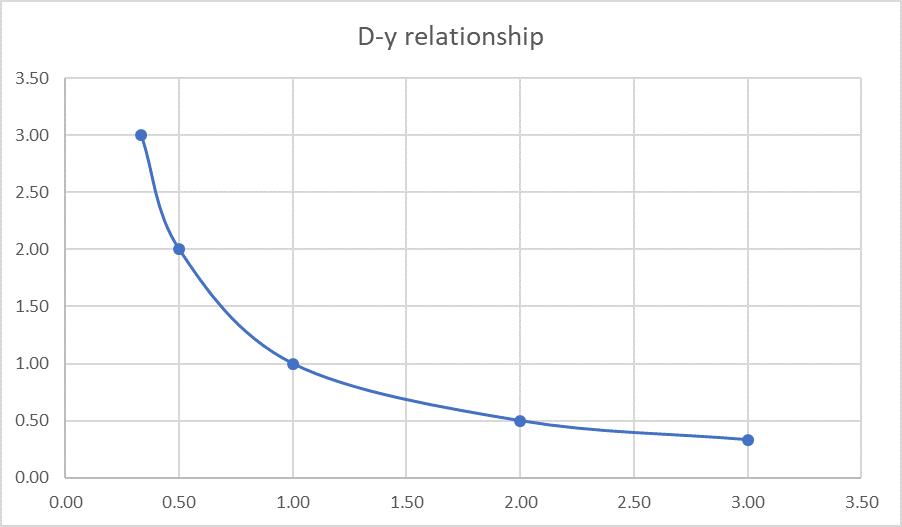
\includegraphics[width=16cm]{img//Newton.PNG}
\caption{牛顿迭代法}
\label{fig:sys.param}
\end{center}
\end{figure}

先根据市场年化率,猜测一个$y_1$,
对曲线上点$(y_1, D_1)$和$(y_0, D_0)$,我们可以求出$Duration = dp/dy$,
逐步调整$y_1$的值,缩小$\Delta y$,
把猜测的值往真实值逼近,
也就是牛顿迭代法。


\subsection{两种模型的对比}
算法总结。
\begin{table}[H]
\begin{adjustwidth}{-3cm}{-3cm}
\begin{center}
\begin{tabular}{|p{.2\textwidth}| p{.8\textwidth}|} \hline
输入 & 给定任意一个coupon bond  \\ \hline
输出 & 该coupon bond的present value,duration以及convexity从市场获得与当前coupon bond相似的其他bond的y,这里的相似主要指的是利率、到期时间等相似,数据来源:彭博社(bloomberg.com)。通过牛顿迭代法找到需要的$y_i$,具体进行几轮牛顿迭代法,找到几个$y_i$,取决于从当前时刻到到期,还要发放利息几次利用上文给出的公式,将$y_i$的具体值带入,求出PV,duration和convexity。  \\ \hline
说明 & 本计算方法的核心在于,我们的利率计算模型。也就是求到期收益率y。对于每一个到期收益率y,有一个现值PV一一对应。对于给定的一个coupon bond,我们在计算其现值PV时,可以有两种处理方法。Y随着时间的变化而变化,可以认为每天都有一个y值(但是不一定每天的y值都不相同,也可能有些日期的y值是相同的。)  \\ \hline
\end{tabular}
\end{center}
\end{adjustwidth}
\end{table}


\paragraph{模型一}
将未来每次发息日发放的利息,折现到当前时刻。例如,假设未来还将发息3次,分别在0.2年、0.7年、1.2年以后,那么我们需要计算出0.2年后对应的到期收益率y,0.7年后的到期收益率y以及1.2年以后的到期收益率y。计算这些y的方法,是通过与给定coupon bound相似的一些coupon bound或者zero coupon bound的y值,来拟合出一条到期收益率y与时间t的关系曲线。通过这种方式,我们将y和t之间的散点图变为了连续函数,使得我们可以得到任何一天的到期收益率y。从而通过将未来的利息及本金折现到当前时刻,得到当前时刻的现值PV。

\paragraph{模型二}
在法一中,我们需要多个y。这里,我们使用一个y来求得当前时刻的现值PV。因为y和PV是一一对应的关系。所以我们通过相似债券的y和PV的关系图,利用牛顿迭代法,直接得到某个到期收益率y对应的现值PV。那么如果知道我输入的coupon bond的在当前时刻y是多少呢?我们可以对一群相似的coupon bond的到期收益率进行加权平均来估计要求的coupon bond的到期收益率y。
